\documentclass{article}
\usepackage{tikz}
\usetikzlibrary{automata,positioning}

\begin{document}

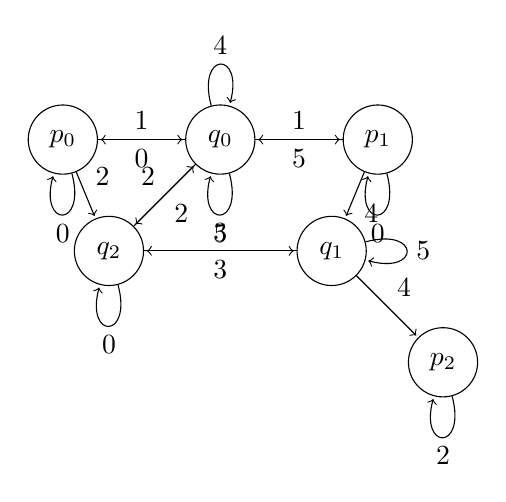
\begin{tikzpicture}[shorten >=1pt,node distance=2cm,on grid,auto]
    \node[state] (p0) {$p_0$};
    \node[state] (q0) [right=of p0] {$q_0$};
    \node[state] (p1) [right=of q0] {$p_1$};
    \node[state] (q1) [below right=of q0] {$q_1$};
    \node[state] (q2) [below left=of q0] {$q_2$};
    \node[state] (p2) [below right=of q1] {$p_2$};

    \path[->]
        (p0) edge node {1} (q0)
             edge node {2} (q2)
             edge [loop below] node {0} ()
        (q0) edge node {0} (p0)
             edge node {1} (p1)
             edge node {2} (q2)
             edge [loop above] node {4} ()
             edge [loop below] node {5} ()
        (p1) edge node {4} (q1)
             edge node {5} (q0)
             edge [loop below] node {0} ()
        (q1) edge node {3} (q2)
             edge node {4} (p2)
             edge [loop right] node {5} ()
        (q2) edge node {3} (q1)
             edge node {2} (q0)
             edge [loop below] node {0} ()
        (p2) edge [loop below] node {2} ();
\end{tikzpicture}

\end{document}